\chapter{Chapter 3} \label{ch:Chapter3}
\section{Switching and Forwarding}
\subsection{Switch}
\begin{definition}
  Dispositivo che interconnette piu' rami di rete differenti per simulare un unica rete.
\end{definition}
Lo switch ha il compito di inoltrare i frame che viaggiano in un segmento agli altri segmenti. Per ogni interfaccia lo switch esegue il protocollo di accesso al mezzo in base al mezzo fisico, la tecnica che viene utilizzata di piu' è la \textbf{store-and-forward}. Ora veniamone il funzionamento:
\begin{itemize}
  \item Lo switch riceve un frame da un'interfaccia. 
  \item Controlla che il frame ricevuto sia corretto; se e' errato lo scarta.
  \item Utilizzando una tabella interna decide dove inviare il frame.
  \item Invia il frame al link scelto.
\end{itemize}
\subsection{Topologia a stella}
L'utilizzo degli swtich aggiunte tra le varie tolopogie di reti quella a stella. I dispositivi sono attaccati a ciascuna porta dello switch le quali sono viste come domini separati quindi non si verificano collisioni tra gli host e lo switch. In collegamenti full duplex i dati possono essere trasferiti tra host e scambiati in ambe le direzioni alla massima velocita'.Bisogna fare attenzione pero' che lo switch ha comunque una banda e memoria limitata.
\subsubsection{Proprieta'}
\begin{itemize}
  \item Uno switch ha un numero fissato di input e output che limita il numero di host che si possono connettere ad uno switch.
  \item Reti piu' grosse possono essere costruite connettendo piu' switch fra loro.
  \item Tutta la rete, per ogni host,appare come una singola rete LAN.
  \item host e altri switch possono essere connessi tramite link point to point. I link possono essere di due tipi: \textit{uplinks} oppure \textit{trunking}.
  \item un ulteriore variante e' quella di utilizzare stakable switches collegati fra loro tramite cavi ad alta velocita'. Questi switch pero' operano come uno solo e non come unita' separate.
  \item L'aggiunta di un nuovo nodo alla rete non implica necessariamente che gli host gia connessi ricevino performance peggiori, ogni host ha il suo link ad uno switch quindi e' possibile che piu' host trasmettano alla max velocita (bandwidth). Il limite di banda trasmissibile e' dato dalla max bandwidth e dalla switching speed. In switch ethernet solitamente varia tra i 10 Gbps e 1M pps (packet per second) fino ad un massimo di 10-20 Tbps.
\end{itemize}
\subsection{Funzionamento switch and forward}
Il primo problema da affrontare e': come si sceglie/decide la porta su cui mandare fuori il frame che arriva. Il lavoro viene fatto dalle switch che,dopo aver controllato che il frame sia corretto, lo inoltra alla porta corretta. Ci sono essenzialmente 3 metodi per prendere questa scelta:
\begin{itemize}
  \item Approccio a datagrammi o \textit{connectionless}
  \item Approccio a circuito virtuale o \textit{connection-oriented}
  \item Source Routing
\end{itemize}
\textbf{Ipotesi:} \\
Ogni host ha un indirizzo globale univoco.\\
\subsubsection{Metodo Connectionless}
Metodo piu' semplice, ogni singolo pacchetto viene trattato in autonomia. Lo switch prende il pacchetto guarda l'header e vede dove mandarlo.
\begin{example}
  Ogni switch tiene all'interno una forwarding table, una tabella che dice a quale porta inoltrare il pacchetto.
\end{example}
\textbf{Caratteristiche:} \\
Un host puo' inviare un pacchetto ovunque e in qualsiasi momento anche se non conosce come e' fatta la rete e se effettivamente il pacchetto arrivera' alla destinazione scelta. Ogni pacchetto viene fowardato indipendentemente, anche se ci sono dei pacchetti precedenti che sono stati inviati alla stessa destinazione (i pacchetti possono seguire piste differente per arrivare alla stessa destinazione). Un errore sul canale o negli switch non causa grossi danni nella rete dato che e' possibile trovare una via alternativa per arrivare a destinazione. \\
\subsubsection{Metodo a circuito virtuale}
E' il duale del connectionless, utilizzato in ambito telefonico e viene anche chiamato connection-oriented. Prima di inviare i dati veri bisogna programmare gli switch intermedi, creare uno stato condiviso all'interno e mantenerlo. \\
Questo processo viene fatto in 3 fasi:
\begin{itemize}
  \item Connection setup: per ogni switch tra la sorgente e la destinazione viene stabilito uno stato di connessione. Questo stato consiste in un entry per la VC table. Questa tabella contiene:
        \begin{itemize}
          \item Virtual Circuit Identifier (VCI): indentifica in modo univoco la connessione a quello switch, questa info sara' contenuta all'interno dell'header dei frame di quella connessione.
          \item Incoming interface: punto di arrivo per i pacchetti di questo VC allo switch.
          \item Outgoing interface: punto di uscita dei pacchetti di questo VC dallo switch.
          \item VCI differente per gestire i pacchetti che escono.
        \end{itemize}
  \item Data Transfer
  \item Connection shutdown
\end{itemize} 
\begin{figure}[H]
  \centering
  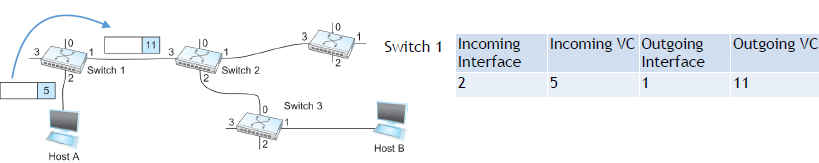
\includegraphics[width=13cm]{figures/circuitoVirtuale.png}
  %\caption{Struttura degli URI. \protect\footnotemark} % Usa \footnotemark qui
  %\label{fig:struttura-uri-dettagliata}
\end{figure}
